\section{Datos}
\label{sec:datos}

\subsection{Descripción de las fuentes de datos a utilizar}

El juego de datos, utilizado para realizar el entrenamiento de la red YOLO, ha sido obtenido de kaggle \footnote{https://www.kaggle.com/felipemuller5/nienaber-potholes-2-complex}. Está compuesto por un total de 1900 imágenes, tomadas desde el interior de un coche, con una resolución de 3680x2760 píxeles (formato 4:3). El juego de datos también consta de un conjunto de ficheros de texto con el etiquetado de las imágenes. Las imágenes se organizan en dos subconjuntos: uno de 1297 imágenes para el entrenamiento y otro de 603 imágenes para la evaluación del modelo. Por cada uno de los subconjuntos de imágenes existe un fichero de texto con el etiquetado de las mismas. Cada una de las líneas del los ficheros de texto contiene las etiquetas de una imagen. La estructura de cada línea es la siguiente:

\begin{lstlisting}[frame=single,basicstyle=\ttfamily\footnotesize]
<RUTA_IMG> <NUMERO_DE_ETIQUETAS>( <X0> <Y0> <ANCHO> <ALTO>)+
\end{lstlisting}

\subsection{Estudio de los datos}

El primer paso que se ha realizado es hacer un estudio de los datos, concretamente se ha hecho un análisis del tamaño de los baches con respecto al tamaño de la imagen. Este es un aspecto importante a tener en cuenta, ya que los algoritmos de detección de objetos son sensibles a este factor y por lo general se comportan peor cuanto más pequeños son los objetos a detectar. Precisamente una de las mejoras que se han conseguido en la última versión de YOLO es la detección de objetos pequeños.

Como se puede observar en la figura \ref{fig:potholesizes}, la mayoría de los baches tienen una anchura inferior a 200 píxeles y una altura inferior a 50 píxeles. Este es un tamaño muy pequeño con respecto a la imagen (3680x2760) y hará difícil su detección.

\begin{figure}[H]
	\centering
	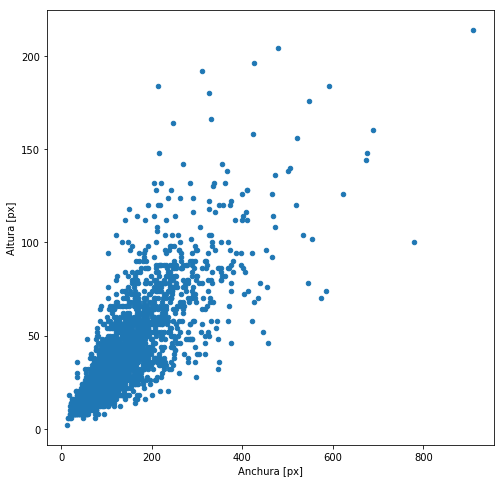
\includegraphics[width=0.7\linewidth]{images/pothole_sizes_scatter_plot.png}
	\caption{Tamaños de los baches en píxeles}
	\label{fig:potholesizes}
\end{figure}

También se ha realizado un estudio de la localización de los baches en las imágenes. Tal y como se ve en la figura \ref{fig:potholeslocations}, los baches están localizados principalmente en el centro de la imagen. La parte inferior se corresponde con el salpicadero del coche y la parte superior se corresponde con paisaje.

\begin{figure}[H]
	\centering
	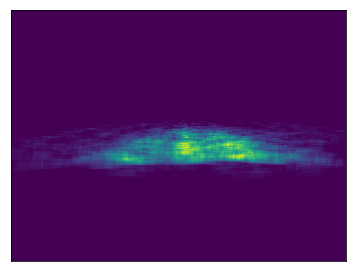
\includegraphics[width=0.7\linewidth]{images/pothole_locations_heatmap.png}
	\caption{Localizaciones de los baches en las imágenes}
	\label{fig:potholeslocations}
\end{figure}

\subsection{Preparación de las imágenes}
\label{subsec:preprocesamiento_de_las_imagenes}

Tanto en la fase de entrenamiento, como para hacer una predicción, las imágenes van a ser redimensionadas al tamaño de la red neuronal, la cual tiene una relación de aspecto 1:1, sin embargo las imágenes del juego de datos tienen una relación de aspecto 4:3.

Para redimensionar una imagen con una relación de aspecto 4:3, y al mismo tiempo, transformarla en una imagen con relación de aspecto 1:1, lo que se hace es redimensionar el lado más grande de la imagen manteniendo la relación de aspecto, es decir, se aplica el mismo factor de redimensionamiento al lado más pequeño. Una vez redimensionada, se rellena con gris la zona superior y la zona inferior de la imagen para cuadrarla. En la figura \ref{fig:imagedirectresize} se muestra un ejemplo gráfico.

\begin{figure}[H]
	\centering
	\begin{subfigure}[h]{0.45\linewidth}
		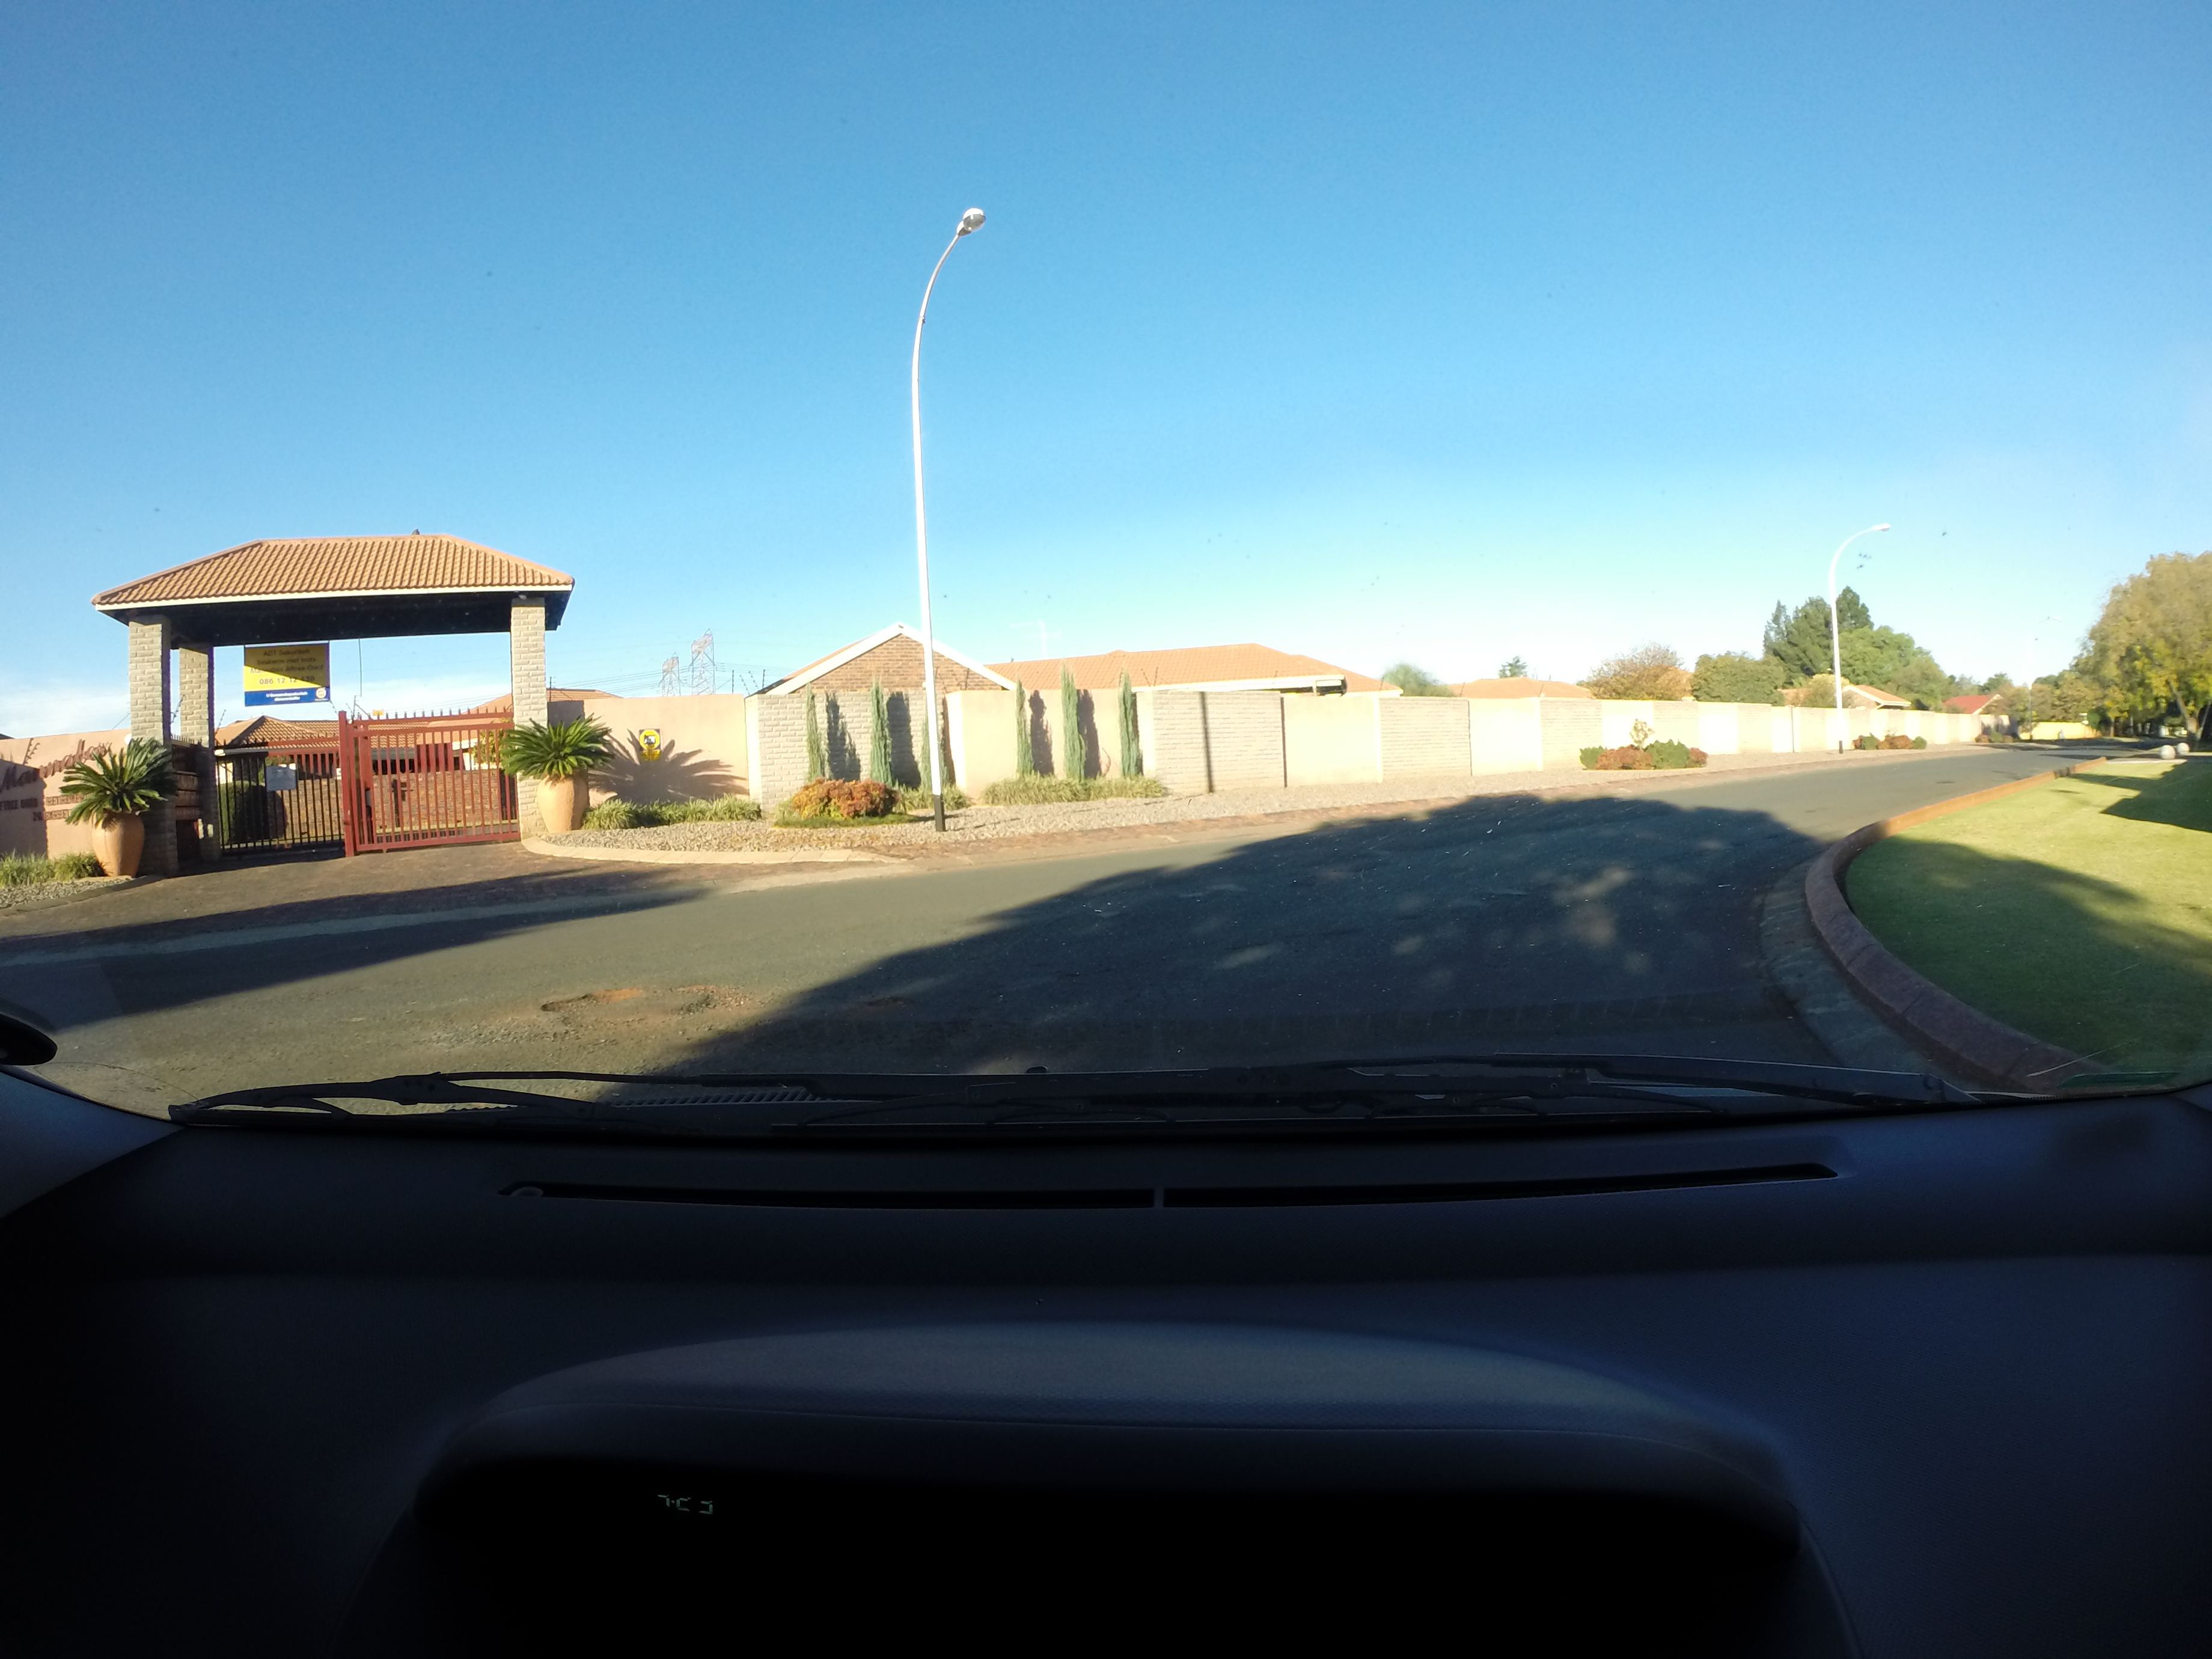
\includegraphics[width=\linewidth]{images/image_direct_resize_before.jpg}
	\end{subfigure}
	\begin{subfigure}[h]{0.45\linewidth}
		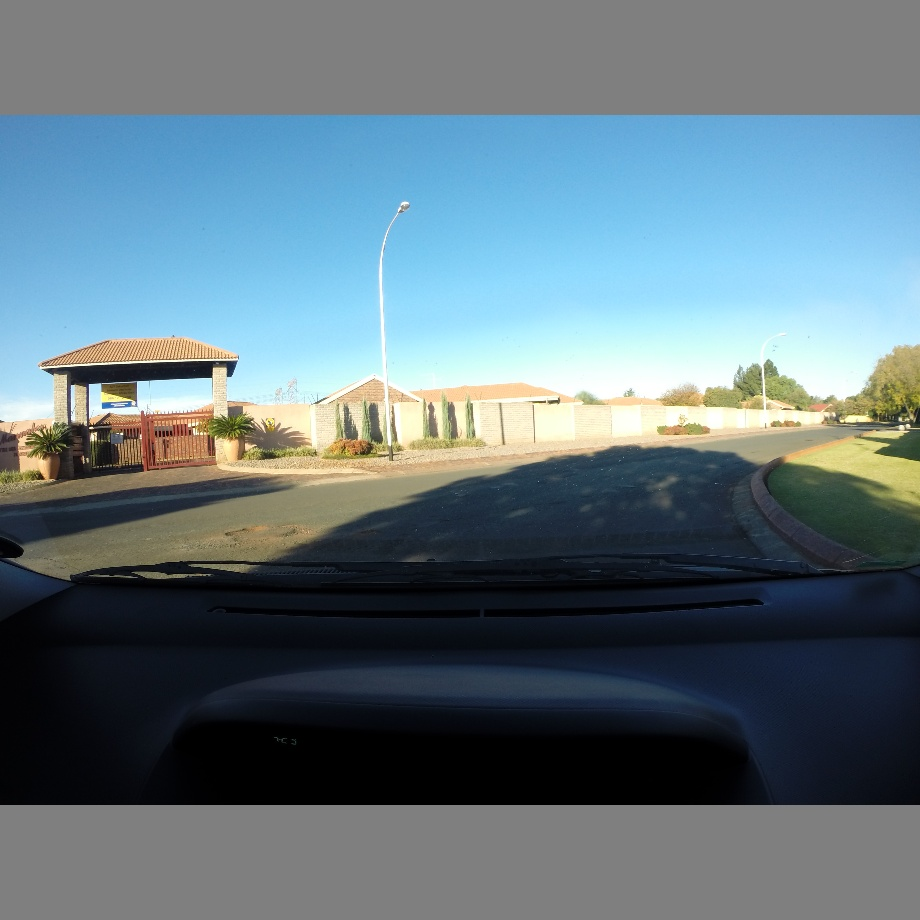
\includegraphics[width=\linewidth]{images/image_direct_resize_after.jpg}
	\end{subfigure}
	\caption{A la izquierda la imagen original redimensionada a tamaño 920x690 px (manteniendo la relación de aspecto 4:3). A la derecha la imagen redimensionada con el relleno para que tenga una relación de aspecto 1:1 (920x920 px)}
	\label{fig:imagedirectresize}
\end{figure}

El redimensionamiento se hace en base al lado más grande de la imagen, que en el ejemplo anterior es la anchura. Para calcular el factor de redimensionamiento, se divide la anchura de la imagen final entre la anchura de la imagen original. En este caso, como se quiere redimensionar la imagen a una anchura de 920 píxeles, el factor de redimensionamiento es: $920 / 3680 = 0.25$. A continuación, se aplica este factor de redimensionamiento a ambos lados de la imagen, resultando en un tamaño de 920x690 píxeles. Por último se calcula el relleno que hace falta a cada lado de la imagen: $(920 - 690) / 2 = 115$.

Siguiendo con este ejemplo, si en la imagen original hubiese un bache de tamaño 160x24 píxeles, y se aplicase este factor de redimensionamiento ($0.25$), el bache redimensionado tendría unas dimensiones de 40x6 píxeles, lo cual sería un tamaño bastante pequeño ya que únicamente tiene 6 píxeles de alto (de los 920 que tiene la imagen).

Sin embargo, si previo al redimensionamiento de la imagen, se recortan los extremos izquierdo y derecho de la imagen, de tal forma que tenga una relación de aspecto 1:1, se consigue que el factor de redimensionamiento sea mayor y que por tanto los baches redimensionados sean también más grandes. Esta técnica tiene un inconveniente, y es que la imagen original se está recortando, por lo que está habiendo una pérdida de información. Este inconveniente no es un impedimento, ya que en el apartado ~\ref{subsec:preprocesamiento_de_las_imagenes} se ha comprobado que la mayor parte de los baches están en el centro de las imágenes, y que recortando los extremos de las mismas la pérdida de información es mínima.

Para aplicar esta técnica, en primer lugar habría que calcular los recortes que hay que hacer a cada lado de la imagen original. Para ello se calcula la diferencia entre la anchura y la altura de la imagen y se divide por dos: $(3680 - 2760) / 2 = 460$. Tras recortar 460 píxeles a cada lado de la imagen se obtiene una imagen de 2760x2760 píxeles. A continuación se calcula el factor de redimensionamiento: $920 / 2760 = 0.333$. Por último se aplica este factor de redimensionamiento a la altura y la anchura de la imagen.

Si aplicásemos este nuevo factor de redimensionamiento al hipotético bache del ejemplo anterior (de tamaño 160x24 píxeles), el tamaño del bache redimensionado sería 53x8, resultando un 75\% más grande.

Todas las imágenes del juego de datos han sido recortadas de esta forma para que al ser redimensionadas, cuando vayan a ser procesadas por el modelo, los baches sean lo más grandes posibles.